\documentclass{beamer}

\mode<presentation>
{
  \usetheme{Madrid}
  \usecolortheme{default}
  \usefonttheme{serif}
  \setbeamertemplate{navigation symbols}{}
  \setbeamertemplate{caption}[numbered]
} 

\usepackage[english]{babel}
\usepackage[utf8x]{inputenc}

\title[]{Macro Attention Indices for Stock Return Predictability}
\author[Arauz, Geiser, Stavropoulos, Tang]{Aaron Arauz Baumender  \\ Michael Adrian Geiser Pasquel \\ Andreas Stavropoulos \\ Zhiyi Tang}
\date{December 2023}

\begin{document}

\begin{frame}
  \titlepage
\end{frame}

\begin{frame}{Abstract}
  We conduct forecasts for equity risk premia utilizing linear and neural network models trained on sets of macroeconomic factors and macroeconomic attention indices. The macroeconomic factors set comprises the 14 features recommended in previous works by Goyal and Welch (2008). The set of macro attention indices includes the eight features constructed by Fisher et al. (2022). Equity risk premia represent the annualized excess return of the one-month S\&P 500 index over the prevailing risk-free rate, approximated by the yield on short-term Treasury Bills. Our analysis focuses on the period between 1985 and 2018, given the availability of the data. However, our results deviate from previous research, suggesting the need for further investigation into the datasets.
  \vspace{1em}

  \textbf{Keywords:} Equity risk premia; Macroeconomic factors; Macro economic attention indices; Neural networks; Financial forecast
\end{frame}

\begin{frame}{Outline}
  \tableofcontents
\end{frame}

\section{Introduction}
\begin{frame}{Introduction}
  \begin{itemize}
    \item \textbf{Background}
      \begin{itemize}
        \item Traditional focus on macroeconomic factors (MEF).
        \item Behavioral finance introduces macro attention indices (MAI) reflecting market sensitivity to information.
        \item Study recognizes interplay between MEF and MAI, and aims to contribute predictive models using linear and neural networks.
      \end{itemize}    
    \item \textbf{Objectives}
      \begin{itemize}
        \item Assess S\&P 500 (GSPC) Equity Risk Premia (ERP) predictive capacity of MEF and MEF using linear regression and neural networks.
      \end{itemize}     
    \item \textbf{Significance of the Study}
      \begin{itemize}
        \item Goes beyond traditional forecasting methods.
        \item Comprehensive analysis with linear and neural network models.
        \item Aims to inform investors, policymakers, and researchers, as well as to enhance understanding of equity market dynamics. 
      \end{itemize}
  \end{itemize}
\end{frame}

\section{Literature Review}
\begin{frame}{Literature Review}
  \begin{itemize}
    \item \textbf{Macroeconomic Factors}
      \begin{itemize}
        \item Insights from Fama and French (1988) and Goyal and Welch (2003) reveal importance of dividends and book value in ERP forecasting.
        \item Recent studies (Lo and Singh, 2003; Gu et al, 2019) use advanced techniques, revealing non linear dynamics.
      \end{itemize}
    \item \textbf{Macro Attention Indices}
      \begin{itemize}
        \item Studies by Andrei and Hasler (2006) and Nikkien et al. (2006) highlight the role in shaping investor sentiment.
        \item Recent research (Ma et al., 2022) emphasizes improved predictive accuracy during market uncertainty.
      \end{itemize}
    \item \textbf{Comparison of Factors and Indices}
      \begin{itemize}
        \item No existing deep comparison of models models, which may offer a more robust framework.
        \item Study uses linear regression models and neural networks for a comprehensive analysis.
      \end{itemize}
  \end{itemize}
\end{frame}

\section{Theoretical Framework}
\begin{frame}{Theoretical Framework}
  \begin{itemize}
    \item \textbf{Market Dynamics Beyond Efficiency}
      \begin{itemize}
        \item Challenges traditional Efficient Market Hypothesis.
        \item Acknowledges anomalies and deviations from efficiency, especially during heightened investor attention.
        \item Highlights the need for alternative frameworks beyond complete market efficiency.
      \end{itemize}
    \item \textbf{Behavioral Finance and Investor Attention}
      \begin{itemize}
        \item Integrates behavioral finance insights into decision-making.
        \item Considers investor attention and herd behavior, leading to overreaction or underreaction.
        \item Accounts for sentiment and attention in forecasting models, recognizing limitations of purely rational assumptions.
      \end{itemize}
    \item \textbf{Neural Networks in Financial Forecasting}
      \begin{itemize}
        \item Utilizes neural networks to capture complex relationships.
        \item Addresses limitations of traditional linear models.
        \item Enhances modeling of interactions between MEF and MAI impacting ERP.
      \end{itemize}  
  \end{itemize}
\end{frame}

\begin{frame}{Theoretical Framework (continued)}
  \begin{itemize}
    \item \textbf{Model Specification}
    \newline
      \begin{itemize}
        \item \textbf{MEF:} Log Dividend-Price $\|$ Log Dividend Yield $\|$ Log Earnings-Price $\|$ Log Dividend-Payout $\|$ Equity Premium Vol $\|$ Book-to-Market Ratio $\|$ Net Equity Expansion $\|$ Treasury Bill Rate $\|$ Long-Term Yield $\|$ Long-Term Return $\|$ Term Spread $\|$ Default Yield Spread $\|$ Default Return Spread $\|$ Inflation
        \newline
        \item \textbf{MAI:} Credit Rating $\|$ Gross Domestic Product $\|$ House Market $\|$ Inflation $\|$ Monetary $\|$ Oil $\|$ Unemployment Rate $\|$ US Dollar
        \newline
        \item \textbf{ERP:} GSPC Equity Risk Premia
      \end{itemize}
  \end{itemize}
\end{frame}

\section{Methodology}
\begin{frame}{Methodology}
  \begin{itemize}
    \item \textbf{Data Management}
    \newline
    Historical data from 1985 to 2018, daily, monthly, and quarterly frequencies. Collected from various repositories, organized chronologically for model training.
    \newline
      \begin{itemize}
        \item \textbf{Data Collection (Raw Data):} MEF and MAI data collected from specific GitHub repositories. GSPC data collected from Yahoo Finance.
        \newline
        \item \textbf{Data Cleaning (Interim Data):} Preprocessing steps applied to address missing values in MAI raw databases.
        \newline
        \item \textbf{Data Processing (Processed Data):} MEF and MAI data undergo processing to construct data for model training. Calculations include transformations and interpolations to derive key macroeconomic factors and attention indexes.
      \end{itemize}
  \end{itemize}
\end{frame}

\begin{frame}{Methodology (continued)}
  \begin{itemize}
    \item \textbf{Model Training}
      \begin{itemize}
        \item Two approaches: linear regression and neural network models.
        \item Linear regression uses the standard equation with gradient descent and Ridge regularization.
        \item Neural network employs traditional feedforward architecture.
        \item Root Mean Squared Error (RMSE) used to assess performance.
      \end{itemize}
    \item \textbf{Comparison and Interpretation}
      \begin{itemize}
        \item Comparative analysis of results from both models.
        \item Evaluation based on RMSE for different combinations of economic data (MAI and MEF) and target variable (1-month GSPC ERP).
        \item Daily and monthly frequencies considered.
      \end{itemize}
  \end{itemize}
\end{frame}

\section{Empirical Analysis}
\begin{frame}{Empirical Analysis}
\begin{itemize}
\item\textbf{The empirical analysis:}
      \begin{itemize}
        \item Involves implementing the models specified in the methodology section to forecast the $1$-month GSPC equity risk premia based on the selected macroeconomic factors (MEF) and macro attention indices (MAI). For this, we use daily and monthly data from both sets of economic data.
        \item The findings from the analysis provide insights into the effectiveness of linear regression and neural network models in predicting equity risk premia and the impact of attention-based metrics.
        \end{itemize}
            \end{itemize}
\end{frame}

\begin{frame}{Empirical Analysis: Data Overview}
  \begin{itemize}
    \item \textbf{Data Overview}
    \begin{itemize}
      \item We used six datasets with their characteristics summarized in the following table:
    \end{itemize}
  \end{itemize}

  \begin{table}[H]
    \centering
    \resizebox{\textwidth}{!}{%
      \begin{tabular}{|c|c|c|c|c|}
        \hline
        \textbf{Dataset} & \textbf{Number of Variables} & \textbf{Frequency} & \textbf{Time Period} & \textbf{Number of Samples} \\ \hline
        MEF Daily & 14 & Daily & 1985/01/02-2018/12/31 & 8523 \\ \hline
        MAI Daily & 8 & Daily & 1985/01/02-2018/12/31 & 8523 \\ \hline
        MKT Daily & 1 & Daily & 1985/01/02-2018/12/31 & 8523 \\ \hline
        MEF Monthly & 14 & Monthly & 1985/01/31-2018/12/31 & 408 \\ \hline
        MAI Monthly & 8 & Monthly & 1985/01/31-2018/12/31 & 408 \\ \hline
        MKT Monthly & 1 & Monthly & 1985/01/31-2018/12/31 & 408 \\ \hline
      \end{tabular}%
    }
    \caption{Description of Datasets used for model training.}
    \label{tab:Datasets}
  \end{table}
\end{frame}

\begin{frame}{Empirical Analysis (continued)}
  \begin{itemize}    
    \item \textbf{Model Implementation}
      \begin{itemize}
        \item \textbf{Linear Regression Model:}
          \begin{itemize}
            \item The linear regression model is implemented using MEF and MAI data as independent variables. The model is trained to establish their linear relationship with GSPC ERP data, the dependent variable.
          \end{itemize}
        \item \textbf{Neural Network Model:}
          \begin{itemize}
            \item The neural network model is implemented using a feedforward neural network architecture. The design of the network includes input layers for MEF and MAI data, hidden layers for capturing non-linear relationships, and an output layer for predicting GSCP ERP. The model is designed to capture the potential non-linear relationship of the datasets.
          \end{itemize}
      \end{itemize}
  \end{itemize}
\end{frame}


\begin{frame}{Empirical Analysis (continued)}
    \begin{itemize}
        \item \textbf{Results}
            \begin{itemize}
                \item The average root mean square error (RMSE) of eight different models (two types of models on four datasets) is tested on ten different random train-test splits of each dataset.
            \end{itemize}
    \end{itemize}

    \begin{table}[H]
        \centering
        \begin{tabular}{|c|c|c|}
          \hline
          \textbf{Model} & \textbf{Input Data} & \textbf{RMSE on Test Set} \\ \hline
          \multirow{4}{*}{Linear Model} & MEF Daily & 53.243 \\ \cline{2-3} 
          & MAI Daily & 54.677 \\ \cline{2-3} 
          & MEF Monthly & 54.307 \\ \cline{2-3} 
          & MAI Monthly & 53.571 \\ \hline
          \multirow{4}{*}{NN Model} & MEF Daily & 51.660 \\ \cline{2-3} 
          & MAI Daily & 51.650 \\ \cline{2-3} 
          & MEF Monthly & 42.794 \\ \cline{2-3} 
          & MAI Monthly & 42.596 \\ \hline
        \end{tabular}
        \caption{Comparison of RMSE of different models}
        \label{tab:PerformanceResults}
    \end{table}
\end{frame}


\begin{frame}{Empirical Analysis (continued)}
  \begin{itemize}
    \item The figures below illustrate disparities between actual and forecasted values generated by our trained linear and neural network models on MAI monthly data.
  \end{itemize}

  \begin{figure}[H]
    \centering
    \begin{minipage}{0.48\textwidth}
      \centering
      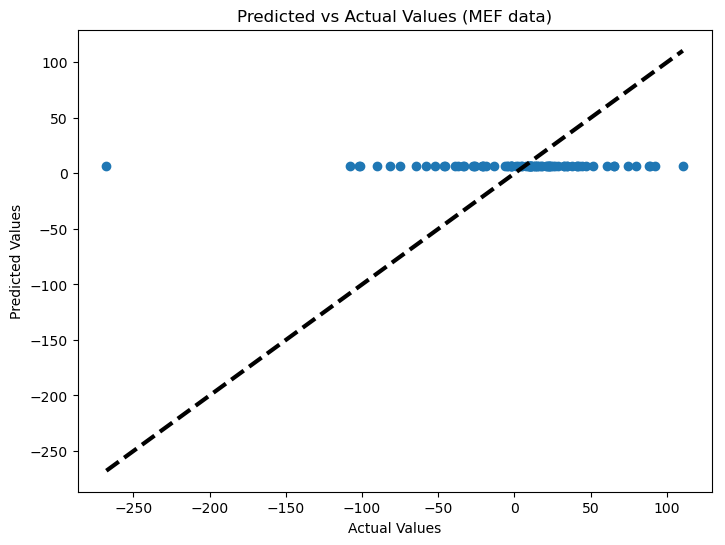
\includegraphics[width=\linewidth]{predvstrue_LM_MAI_M.png}
      \caption{Linear Model Prediction}
      \label{fig:linear_prediction}
    \end{minipage}\hfill
    \begin{minipage}{0.48\textwidth}
      \centering
      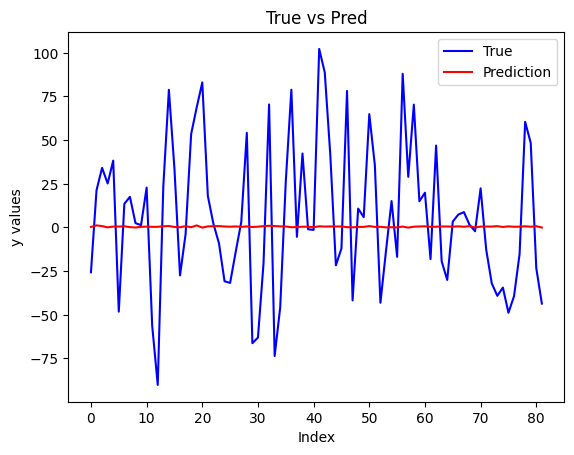
\includegraphics[width=\linewidth]{predvstrue_NN_MAI_M.png}
      \caption{Neural Network Model Prediction}
      \label{fig:nn_prediction}
    \end{minipage}
  \end{figure}
\end{frame}

\begin{frame}{Empirical Analysis (continued)}
  \begin{figure}
    \centering
    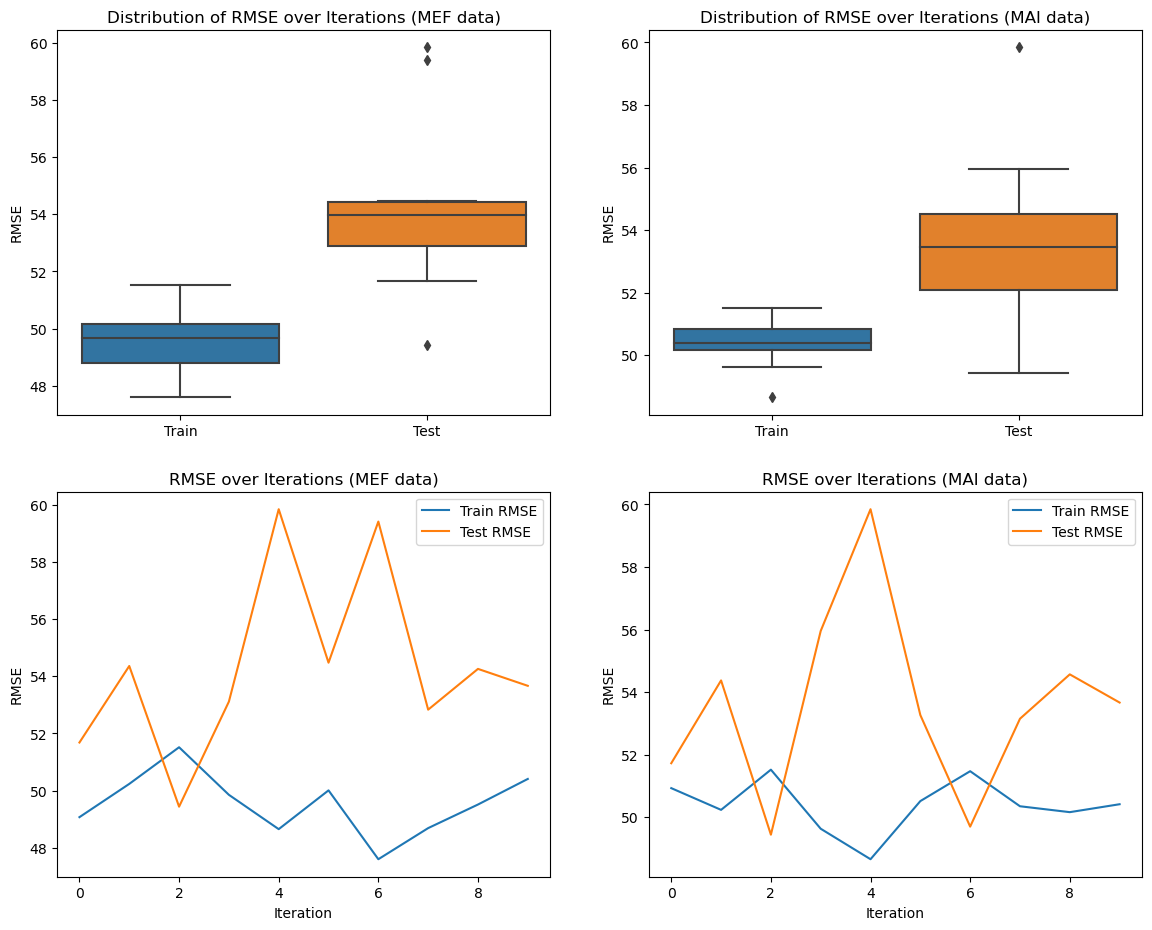
\includegraphics[width=0.70\textwidth]{Distribution of RMSE_Linear_M.png}
    \caption{Distribution of RMSE over iterations, linear models on monthly data.}
    \label{fig:linear_prediction_ii}
  \end{figure}
\end{frame}

\begin{frame}{Empirical Analysis (continued)}
  \begin{itemize}
    \item Distribution of RMSE over iterations, NN models on monthly data.
  \end{itemize}

  \begin{figure}[H]
    \centering
    \begin{minipage}{0.48\textwidth}
      \centering
      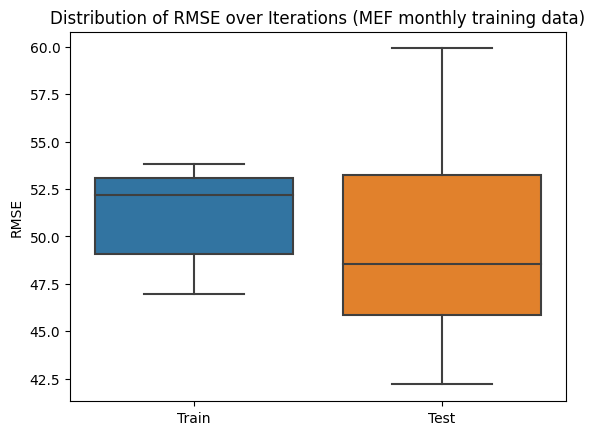
\includegraphics[width=\linewidth]{Distribution of RMSE_NN_MEF_M.png}
      \caption{MEF monthly.}
      \label{fig:linear_prediction}
    \end{minipage}\hfill
    \begin{minipage}{0.48\textwidth}
      \centering
      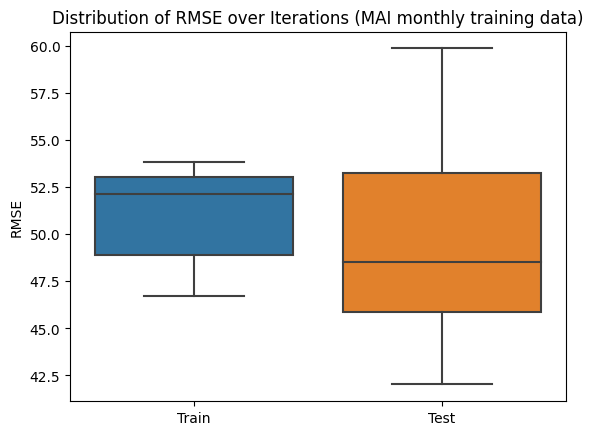
\includegraphics[width=\linewidth]{Distribution of RMSE_NN_MAI_M.png}
      \caption{MAI monthly.}
      \label{fig:nn_prediction}
    \end{minipage}
  \end{figure}
\end{frame}

\begin{frame}{Empirical Analysis (continued)}
    \begin{itemize}
        \item \textbf{Comparison and Interpretation}
        \begin{itemize}
            \item \textbf{Model Selection}
            \begin{itemize}
                \item Neural network models outperform linear regression models across all datasets with an approximately 17-unit lower RMSE. 
                \item Their superior predictive accuracy makes them robust for real-world applications.
            \end{itemize}
            
            \item \textbf{Data Selection}
            \begin{itemize}
                \item Linear models provide insights into individual factors' impact on equity risk premia through coefficient examination. 
                \item An interactive Shiny app allows users to visualize the impact of various features and temporal ranges. 
                \item The app supports flexible selections of MEF and MAI variables, temporal spans (from 1.1.1985 to 31.12.2018), and frequencies (daily, monthly, quarterly).
            \end{itemize}
        \end{itemize}
    \end{itemize}
\end{frame}


\begin{frame}{Empirical Analysis (continued)}
  \begin{itemize}
    \item In the first case, quarterly data between 1.1.1985 and 31.12.2018 of MEF Log Dividend-Price (solid blue), MEF Log Dividend Yield (dashed blue), MAI Credit Rating (dashed green), and MKT GSPC (solid red) are selected.
  \end{itemize}
    \begin{figure}[H]
        \centering
        \begin{minipage}{.80\textwidth}
            \centering
            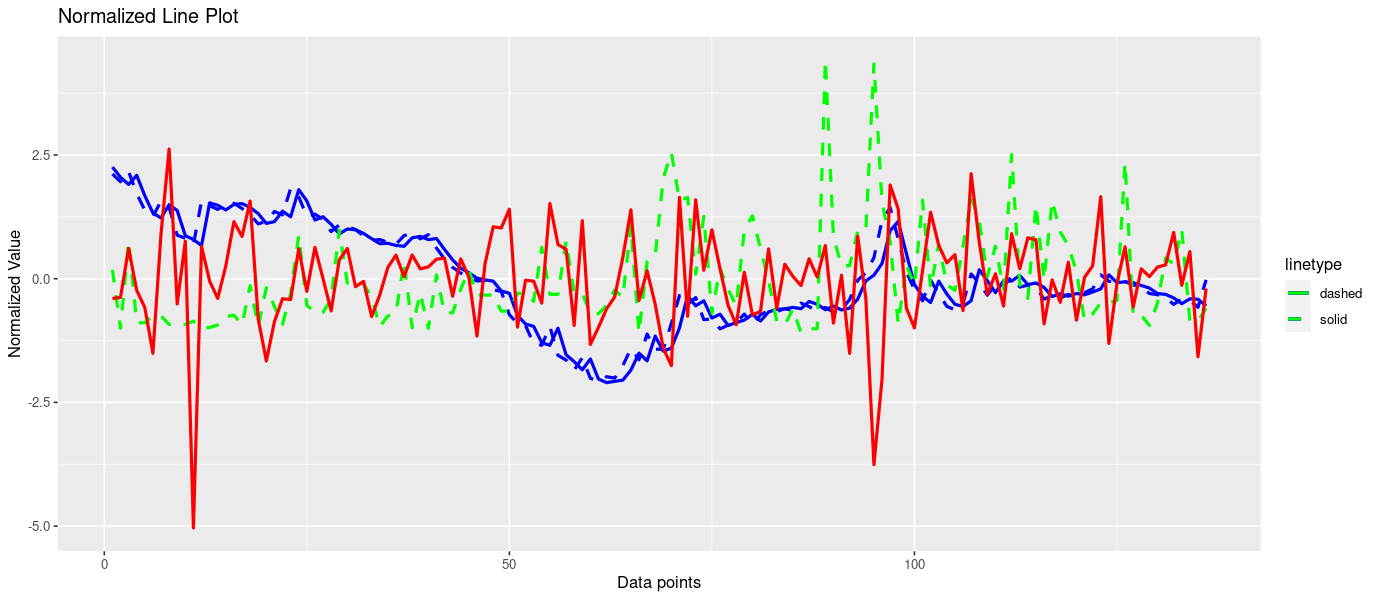
\includegraphics[width=\linewidth]{MEF_dpdy_MAI_cr.png}
            \caption{Shiny app variable selection outcome, Case 1.- \href{https://baumender11.shinyapps.io/Alpha/}{Interactive Shiny App}}
            \label{fig:linear_prediction}
        \end{minipage}
    \end{figure}
\end{frame}

\begin{frame}{Empirical Analysis (continued)}
  \begin{itemize}
    \item In the second case, quarterly data between 1.1.1985 and 31.12.2018 of MEF Log Dividend-Price (solid blue), MEF Log Dividend Yield (dotted blue), MEF Log Earnings-Price (dashed blue), MAI Credit Rating (dotted green), MAI Gross Domestic Product (solid green), and MKT GSCP (solid red) are selected.
  \end{itemize}
    \begin{figure}[H]
        \centering
        \begin{minipage}{.80\textwidth}
            \centering
            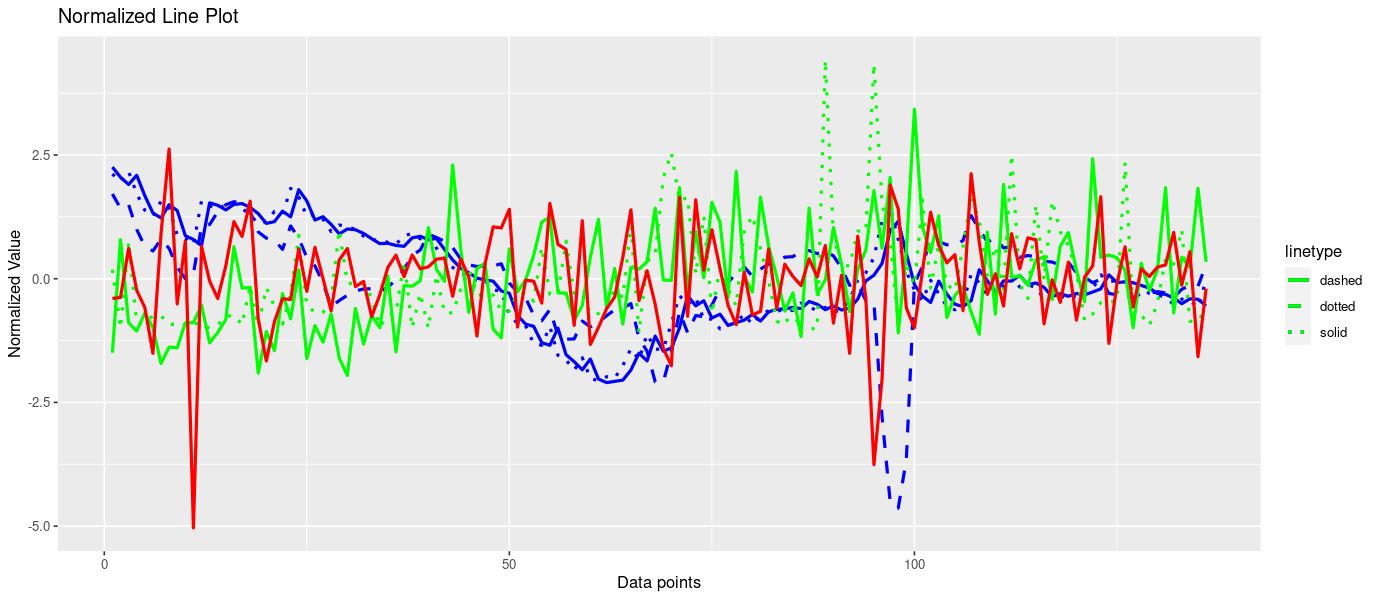
\includegraphics[width=\linewidth]{MEF_dpdyep_MAI_crgdp.png}
            \caption{Shiny app variable selection outcome, Case 2.- \href{https://baumender11.shinyapps.io/Alpha/}{Interactive Shiny App}}
            \label{fig:linear_prediction}
        \end{minipage}
    \end{figure}
\end{frame}

\begin{frame}{Empirical Analysis (continued)}
  \begin{itemize}
    \item{ Correlation heatmaps, MEF data between, 1.1.1985 and 31.12.2018.} 
  \end{itemize}

  \begin{figure}[H]
    \centering
    \begin{minipage}{0.32\textwidth}
      \centering
      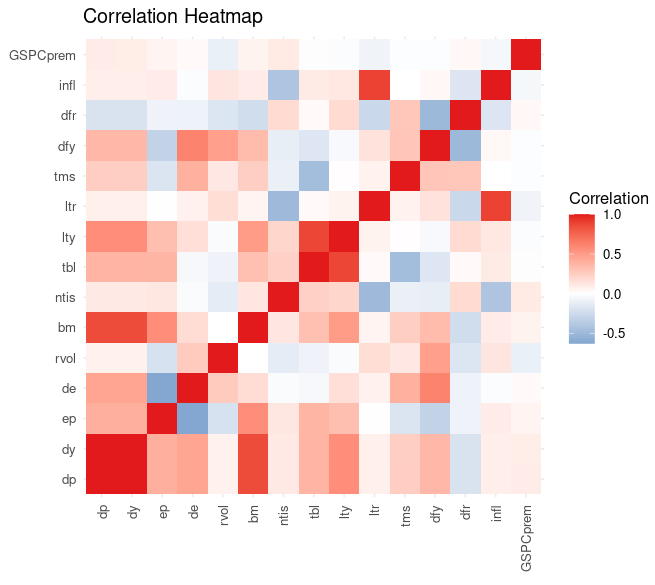
\includegraphics[width=\linewidth]{Cormap_MEF_Daily_85.png}
      \caption{MEF daily.}
      \label{fig:linear_prediction}
    \end{minipage}\hfill
    \begin{minipage}{0.32\textwidth}
      \centering
      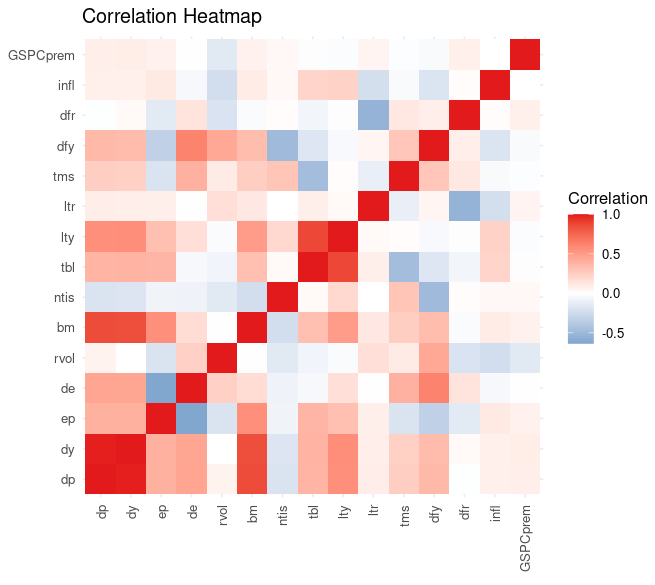
\includegraphics[width=\linewidth]{Cormap_MEF_Monthly_85.png}
      \caption{MEF monthly.}
      \label{fig:nn_prediction}
    \end{minipage}\hfill
    \begin{minipage}{0.32\textwidth}
      \centering
      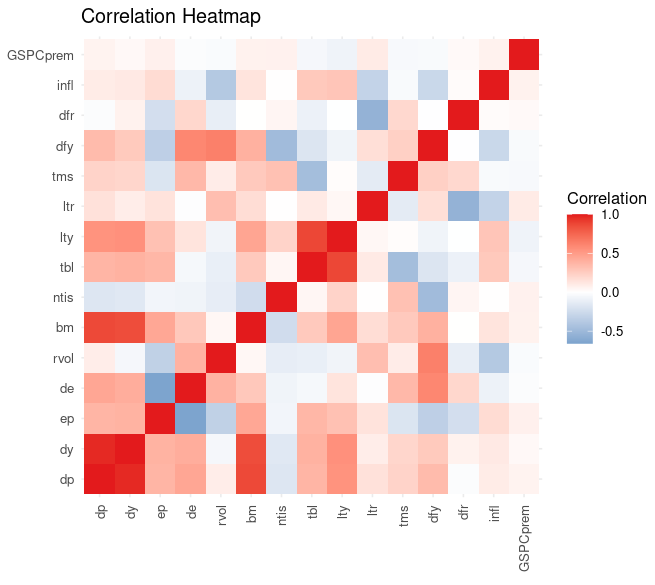
\includegraphics[width=\linewidth]{Cormap_MEF_Quarterly_85.png} 
      \caption{MEF quarterly.}
      \label{fig:third_prediction}
    \end{minipage}
  \end{figure}
\end{frame}

\begin{frame}{Empirical Analysis (continued)}
  \begin{itemize}
    \item{ Correlation heatmaps, MEF data between, 1.1.2000 and 31.12.2018}
  \end{itemize}

  \begin{figure}[H]
    \centering
    \begin{minipage}{0.32\textwidth}
      \centering
      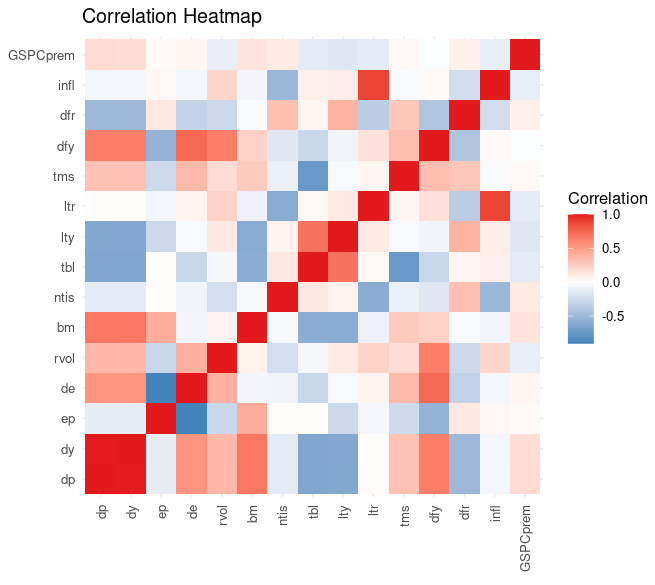
\includegraphics[width=\linewidth]{Cormap_MEF_Daily_00.png}
      \caption{MEF daily.}
      \label{fig:linear_prediction}
    \end{minipage}\hfill
    \begin{minipage}{0.32\textwidth}
      \centering
      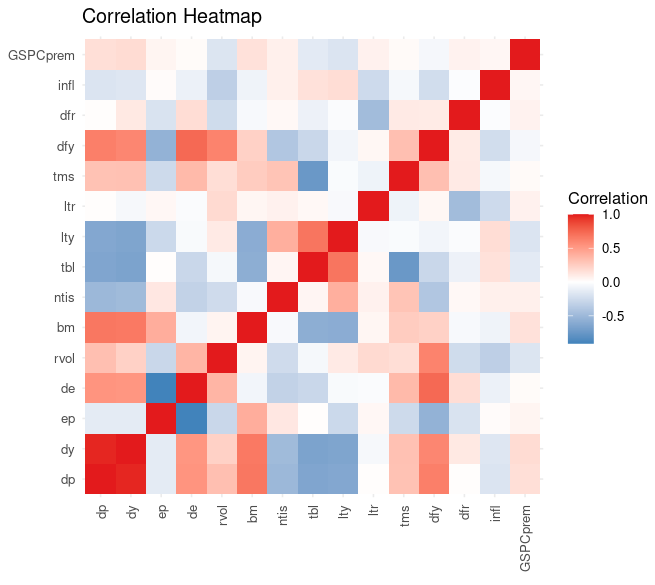
\includegraphics[width=\linewidth]{Cormap_MEF_Monthly_00.png}
      \caption{MEF monthly.}
      \label{fig:nn_prediction}
    \end{minipage}\hfill
    \begin{minipage}{0.32\textwidth}
      \centering
      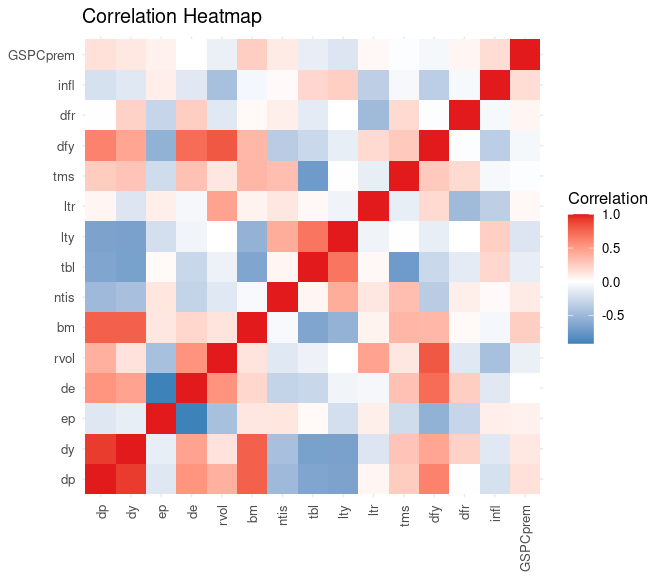
\includegraphics[width=\linewidth]{Cormap_MEF_Quarterly_00.png} 
      \caption{MEF quarterly.}
      \label{fig:third_prediction}
    \end{minipage}
  \end{figure}
\end{frame}

\section{Discussion}
\begin{frame}{Discussion}
  \begin{itemize}
    \item \textbf{Practical Implications} 
    \begin{itemize}
        \item Neural network models outperform linear models, and both MEF and MAI data equally impact prediction quality, challenging previous conclusions.
    \end{itemize}
    \item \textbf{Limitations}
    \begin{itemize}
        \item Despite superior mean RMSE for neural networks, notable variability exists.
    \end{itemize}
    \item \textbf{Future Research Directions}
    \begin{itemize}
        \item Model improvement is needed, considering the time series correlation characteristics of equity risk premia.
        \item Exploring differences between MAI and MEF in capturing macroeconomic influences on equity risk premia can offer valuable insights into nuanced dynamics.
    \end{itemize}
  \end{itemize}
\end{frame}

\section{Conclusion}
\begin{frame}{Conclusion}
  \begin{itemize}
    \item \textbf{Findings}
    \begin{itemize}
        \item Neural network models outperform linear regression across datasets, offering robust predictive capabilities for real-world applications.
        \item Eight models, including linear and neural networks, are trained on three datasets.
    \end{itemize}     
    \item \textbf{Limitations} 
    \begin{itemize}
        \item Despite neural network superiority, observed RMSE variability indicates challenges in identifying causal relationships.
    \end{itemize}
    \item \textbf{Future Research}
      \begin{itemize}
        \item Enhance model structure by considering time series correlation in equity risk premia.
        \item Explore more advanced modeling, starting with neural networks and incorporating macroeconomic features.
        \item Investigate differences in capturing macroeconomic influence between MAI and MEF.
      \end{itemize}
  \end{itemize}
\end{frame}

\section{References}
\begin{frame}{References}
  \begin{itemize}
    \item Fama and French (1988): \emph{Dividend Yields and Expected Stock Returns}
    \item Goyal and Welch (2003): \emph{Predicting the Equity Premium with Dividend Ratios}
    \item Lo and Singh (2003): \emph{Deep-learning models for forecasting financial risk premia and their interpretations}
    \item Gu, Kelly, and Xiu (2019): \emph{Empirical Asset Pricing via Machine Learning}
    \item Andrei and Hasler (2012): \emph{Investors’ Attention and Stock Market Volatility}
    \item Nikkinen, Omran, Sahlström, and Äijö (2006): \emph{Global stock market reactions to scheduled U.S. macroeconomic news announcements}
    \item Ma, Lu, Liu, and Huang (2022): \emph{Macroeconomic attention and stock market return predictability}
  \end{itemize}
\end{frame}
\end{document}
